%%%%%%%%%%%%%%%%%%%%%%%%%%%%%%%%%%%%%%%%%%%%%%%%%%%%%%%%%%%%%%%%%%%%%%%%%%%%%%%
%% Machine Learning IrOx OER Paper
%% Added in Overleaf | RF | 190720
%%%%%%%%%%%%%%%%%%%%%%%%%%%%%%%%%%%%%%%%%%%%%%%%%%%%%%%%%%%%%%%%%%%%%%%%%%%%%%%

% | - __latex_setup__
\documentclass[journal=jacsat,manuscript=article]{achemso}
\usepackage[version=3]{mhchem} % Formula subscripts using \ce{}
\usepackage{subfig}
\usepackage{multirow}
\usepackage[table,xcdraw]{xcolor}
\usepackage{hhline}
\usepackage{svg}  % 181208 | RF | Added to include svg files
% __|

% - Author List ***************************************************************
%%%%%%%%%%%%%%%%%%%%%%%%%%%%%%%%%%%%%%%%%%%%%%%%%%%%%%%%%%%%%%%%%%%%%%%%%%%%%%%
%%
%%
%%
%%%%%%%%%%%%%%%%%%%%%%%%%%%%%%%%%%%%%%%%%%%%%%%%%%%%%%%%%%%%%%%%%%%%%%%%%%%%%%%


% | - @Raul Flores
\author{Raul A. Flores}
\affiliation[SUNCAT]{
  SUNCAT Center for Interface Science and Catalysis,
  Department of Chemical Engineering,
  Stanford University,
  Stanford 94305,
  California,
  USA
  }
\email{flores12@stanford.edu}
% __|

% | - @Christopher Paolucci
\author{Christopher Paolucci}
\affiliation[UVA]
{
  Department of Chemical Engineering,
  University of Virginia,
  Charlottesville,
  Virginia 22903,
  United States
  }
\email{cp9wx@virginia.edu}
% __|

% | - Ankit Jain
\author{Ankit Jain}
\affiliation[DTU]
{
  Department of Physics,
  Technical University of Denmark,
  Lyngby,
  Denmark
  }
\email{temp_temp_ankits_email_address_temp_temp@dtu.dk}
% __|

% | - Ziyun Wang
% \author{Zhyun}
% \affiliation[SUNCAT]
% {
% SUNCAT Center for Interface Science and Catalysis,
% Department of Chemical Engineering,
% Stanford University,
% Stanford,
% California,
% United States
% }
% \email{temp_temp_ankits_email_address_temp_temp@dtu.dk}s
% __|


\author{Kirsten T. Winther}
\affiliation[SUNCAT]{
  SUNCAT Center for Interface Science and Catalysis,
  Department of Chemical Engineering,
  Stanford University,
  Stanford 94305,
  California,
  USA
  }



% | - Muratahan Aykol
\author{Muratahan Aykol}
\affiliation[TRI]
{
  Toyota Research Institute,
  Los Altos,
  CA 94022,
  USA
  }
\email{muratahan.aykol@tri.global}
% __|

% | - Jens Norskov
\author{Jens K. N{\o}rskov}
\affiliation[DTU]
{
  Department of Physics,
  Technical University of Denmark,
  Lyngby,
  Denmark
  }
\email{jkno@dtu.dk}
% __|

% | - @Michal Bajdich
\author{Michal Bajdich}
\affiliation[SLAC]{
  SUNCAT Center for Interface Science and Catalysis,
  SLAC National Accelerator Laboratory,
  Menlo Park,
  CA 94025,
  USA
  }
\email{bajdich@slac.stanford.edu}
% __|

% | - Thomas Bligaard
\author{Thomas Bligaard}
\affiliation[SLAC]{
  SUNCAT Center for Interface Science and Catalysis,
  SLAC National Accelerator Laboratory,
  Menlo Park,
  CA 94025,
  USA
  }
\email{bligaard@stanford.edu}
% __|


% - Custom Macros *************************************************************
%%%%%%%%%%%%%%%%%%%%%%%%%%%%%%%%%%%%%%%%%%%%%%%%%%%%%%%%%%%%%%%%%%%%%%%%%%%%%%%
% Latex Macros
%%%%%%%%%%%%%%%%%%%%%%%%%%%%%%%%%%%%%%%%%%%%%%%%%%%%%%%%%%%%%%%%%%%%%%%%%%%%%%%

% Chris commenting command
\newcommand{\chris}[1]{\textcolor{red}{#1}}
\newcommand{\comment}[1]{\textcolor{red}{\textbf{#1}}}


% #########################################################
% Chemical formulas #######################################
% IrOx, IrO3, IrO2
\def \IrOx {IrO\textsubscript{x}\xspace}
\def \IrOthree {IrO\textsubscript{3}\xspace}
\def \IrOtwo {IrO\textsubscript{2}\xspace}

% RhO2
\def \RhOtwo {RhO\textsubscript{2}\xspace}

% rutile-IrO2, alpha-IrO3, rutile-IrO3, beta-IrO3
\def \rIrOtwo {R-\ce{IrO_2}\xspace}
\def \aIrOthree {$\alpha$-\ce{IrO_3}\xspace}
\def \rIrOthree {R-\ce{IrO_3}\xspace}
\def \bIrOthree {$\beta$-\ce{IrO_3}\xspace}

% Aqueous IrO4- phase
\def \IrOfourm {\ce{IrO_{4}^{-}}\xspace}

% AB2 and AB3 (ABO3 too)
\def \ABtwo {AB\textsubscript{2}\xspace}
\def \ABthree {AB\textsubscript{3}\xspace}
\def \ABOthree {AB\textsubscript{3}\xspace}

% #########################################################
% Adsorption energies #####################################

% ΔE_OH, ΔE_O, ΔE_OOH
\def \DEOH {$\Delta$E\textsubscript{OH}\xspace}
\def \DEO {$\Delta$E\textsubscript{O}\xspace}
\def \DEOOH {$\Delta$E\textsubscript{OOH}\xspace}

% ΔG_OH, ΔG_O, ΔG_OOH
\def \DGOH {$\Delta$G\textsubscript{OH}\xspace}
\def \DGO {$\Delta$G\textsubscript{O}\xspace}
\def \DGOOH {$\Delta$G\textsubscript{OOH}\xspace}

% ΔG_O-ΔG_OH
\def \DGOmOH {$\Delta$G\textsubscript{O}-$\Delta$G\textsubscript{OH}}


% #########################################################
% Enthalpy of formation ΔH_f ##############################
\def \DHf {$\Delta$H\textsubscript{f}\xspace}
\def \DGf {$\Delta$G\textsubscript{f}\xspace}

% #########################################################
% V vs RHE notation #######################################
\def \VRHE {$V\textsubscript{RHE}$\xspace}

% Angstrom
\newcommand{\angstrom}{\textup{\AA}}

% Tilde ~
\newcommand{\mytilde}{\raise.17ex\hbox{$\scriptstyle\mathtt{\sim}$}}


% Article Title ***************************************************************
\title[ML discovered IrOx phases]{
  Machine-Learning Discovery of Highly Oxidized \IrOx Phases}

\begin{document}

% | - TOC Figure
\begin{tocentry}
\begin{center}
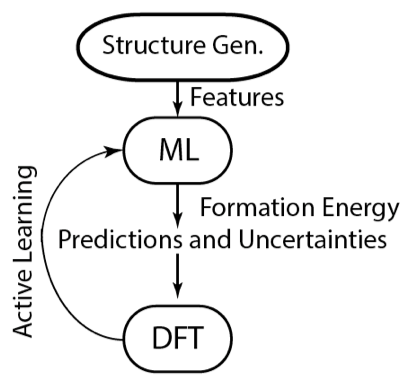
\includegraphics[height=3.5cm]{02_figures/Surrogate_model}
\end{center}
\end{tocentry}
% __|

% #############################################################################
% - MAIN DOCUMENT *************************************************************

% - 00 | Abstract *************************************************************
\begin{abstract}
%%%%%%%%%%%%%%%%%%%%%%%%%%%%%%%%%%%%%%%%%%%%%%%%%%%%%%%%%%%
% Abstract %%%%%%%%%%%%%%%%%%%%%%%%%%%%%%%%%%%%%%%%%%%%%%%%
% %%%%%%%%%%%%%%%%%%%%%%%%%%%%%%%%%%%%%%%%%%%%%%%%%%%%%%%%%
%
%%%%%%%%%%%%%%%%%%%%%%%%%%%%%%%%%%%%%%%%%%%%%%%%%%%%%%%%%%%

%| - MY OLD VERSION
% %
% Machine learning (ML) based surrogate models have become an increasingly common tool in the field computational materials discovery to overcome the relative expense of \latin{ab-initio} density functional theory (DFT).
% %
% Training such models on expansive DFT data sets has been used to discover new materials in the vast space of material compositions.
% %
% % COMBAK This is probably too strong
% However, surrogate model applications to the structural space of bulk crystals, \latin{i.e.} polymorphs, remain relatively unexplored.
% %
% Herein, we report on an active learning (AL) framework that searches for the most stable polymorph of a chemical space by utilizing a surrogate model which is sequentially updated on the fly with generated DFT data.
% %
% The model searches within a candidate data set of crystal motifs sourced from publicly available materials databases.
% %
% We demonstrate the efficacy of this AL-accelerated methodology by discovering the most stable polymorphs of \IrOtwo and \IrOthree within the candidate space with DFT calculations of only a fraction of the candidate space.
% % 7 out of the 10 most stable crystal structures for \IrOtwo and \IrOthree with less than 50 DFT calculations.
% %
% % COMBAK TODO Update number of unique polymorphs discovered to something more meaningful
% % Let's report how many meta-stable IrO2/3 we discovered, much better than how it is currently phrased
% For \IrOtwo, we reaffirm the rutile phase as the globally stable polymorph, while also finding \mytilde200 polymorphs that are within the synthesizability limit.
% %
% For \IrOthree we discovered ~70 unique metastable polymorphs, with \mytilde20 that are more stable than anything previously reported.
% %
% The globally stable polymorph of \IrOthree is a FeF\textsubscript{3} structure type polymorph with a space group number of 167.
% %
% % There are 10 IrO3 polymorphs within 0.2 eV/atom of the lowest structure and 5 IrO3 polymorphs within 0.1 eV/atom of the lowest structure
% % Of these 10, how many were unknown? Maybe 8ish? TODO double check
% %
% %For \IrOthree, we discover 10 previously unknown polymorphs, and the most stable
% %$\alpha$-AlF\textsubscript{3} type and a rutile-like \IrOthree structure with stabilities lower than 0.2 per atom than anything known to date.
% %
% Based on the above results, we constructed a revised bulk Pourbaix diagram of the Ir-H\textsubscript{2}O system by including \IrOthree, and show that our \aIrOthree phase is the dominant and fully stable phase under acidic oxygen evolution reaction (OER) conditions.
% %
% % COMBAK "the OER" or just "OER"
% Using a thermodynamic criteria for the activity towards the OER we find that the above stable \IrOthree polymorphs have significantly lower theoretical overpotentials than the rutile \IrOtwo phase.
% %
% This elevated catalytic activity is due to the weaker and more ideal binding of the OER intermediates on the more oxidized \IrOthree surfaces.
% %
% % TODO Less cheesy closing thoughts
% This work opens up the possibility of drastically accelerating the discovery of novel crystal structure motifs and has implications towards high through-put catalyst discovery efforts.

%__|





%
Materials science primarily studies the relationship between the structure and functionality of materials,
where the knowledge of viable polymorphic forms of crystals at a given chemical composition plays an indispensable role.
%
Machine-learning based surrogate models have the potential to accelerate this process of creating the knowledge-base for materials polymorphs for target applications in under-explored chemistries.
%
Herein, we report on a sequential, active-learning (AL) accelerated ab-initio study for the identification of novel and stable \IrOx (x=2 or 3) polymorphs,
and the subsequent thermochemical analyses of the activity of these discovered structures towards the oxygen evolution reaction (OER).
%
We demonstrate that compared to a random search,
the AL framework at more than doubles the efficiency of using DFT to find stable polymorphs out of a large array of prototypical structures.
%
We find nearly \num{200} and \num{70} unique polymorphs within the thermodynamic synthesizability limits of \IrOtwo and \IrOthree, respectively,
while validating the rutile ground state for the former and finding a new \ce{FeF_{3}}-like ground state for the latter (\aIrOthree).
%
An analysis of the structural properties of these metastable polymorphs reveals that octahedral local coordination environments are preferred for all low energy structures.
%
Subsequent Pourbaix and thermochemical analyses with this \aIrOthree phase show that it is fully stable under acidic OER conditions,
and delivers lower theoretical overpotentials compared to \rIrOtwo due to weaker and more ideal binding of the OER intermediates on its oxidized surfaces.

\end{abstract}

% - 01 | Introduction *********************************************************
\section{Introduction}
%%%%%%%%%%%%%%%%%%%%%%%%%%%%%%%%%%%%%%%%%%%%%%%%%%%%%%%%%%%%%%%%%%%%%%%%%%%%%%%
% Introduction %%%%%%%%%%%%%%%%%%%%%%%%%%%%%%%%%%%%%%%%%%%%%%%%%%%%%%%%%%%%%%%%
% %%%%%%%%%%%%%%%%%%%%%%%%%%%%%%%%%%%%%%%%%%%%%%%%%%%%%%%%%%%%%%%%%%%%%%%%%%%%%
%
% Key points:
%   * Materials are composed of their "stoichiometry" and their "structure"
%   * 3N dimensional Cartesian space of coordinates is prohibitelvey large
%   * Our candidate space generation leverages symmetry to produce a set of
%     structurally unique and well distributed (across the high dim. 3N space)
%     polymorphs
%   * Mention other methods for bulk crystal structure Discovery
%     - simulated annealing
%     - paper that Hammer put out (R58)
%%%%%%%%%%%%%%%%%%%%%%%%%%%%%%%%%%%%%%%%%%%%%%%%%%%%%%%%%%%%%%%%%%%%%%%%%%%%%%%



% ################################# Paragraph #################################
% %%%%%%%%%%%%%%%%%%%%%%%%%%%%%%%%%%%%%%%%%%%%%%%%%%%%%%%%%%%%%%%%%%%%%%%%%%%%%
% * General intro into problem, give proper context
% * Make the point that structure has been all but ignored in recent years by the big-data/ML material science community (OQMD MP as examples)
%
% OUTLINE:
%  * Solving for crystal structures in a generally difficult problem
%  * It's an important problem to solve because all chemical/physical properties of a material are fundementally linked to the atomic structure.
%  * Although we've seen a lot of work in the past ~10 years from material science groups leveraging recent advances in big-data, ML, cheaper computational resources, high-throughput screening, materials databases, etc.
%    * Most of the focus has been on exploring compositionas and not structure
% %%%%%%%%%%%%%%%%%%%%%%%%%%%%%%%%%%%%%%%%%%%%%%%%%%%%%%%%%%%%%%%%%%%%%%%%%%%%%
% | - Paragraph start
% TODO this intro sentence will be a reference dump for literature in crystal structure prediction
Predicting the thermodynamically favorable crystal structures for an arbitrary inorganic system remains a challenging problem in computational material science.\cite{Woodley2008}
%
% Experimentally synthesized inorganic materials often conform to the global minimum energy structure (or similarly stable meta-stable phases).
%
When simulations are used to guide the search for new materials, the stable and meta-stable crystal structures, \latin{i.e.} polymorphs,  above the convex hull of stability must be known in order to predict the material properties.\cite{}
%
% Structure vs. composition enumeration (composition done to death)
% Give example of how over represented some motifs are
% 188,000 systems with identical prototype ABO2 perovskites structure (~50 %)
% Not sure what to cite for this, example is sufficient
Although there have been numerous examples in recent years of machine learning algorithms applied towards the prediction of formation energies of large \latin{ab-initio} data sets,
these data sets are biased towards common structures and varying composition space.\cite{}
% NUMBER
For example, roughly half of the entries (\mytilde\num{200000}) in The Open Quantum Materials Database (OQMD) correspond to ternary-alloy combinations in the same close-packed cubic structure.\cite{Kirklin2015}
%have identical structures corresponding to ABO3 Perovskites.
% Should we say that enumerating comp. is easy and struct. is hard?
As such, these efforts have been primarily concerned with the enumeration of composition (elemental identity and stoichiometries) and less so with the exploration of structural diversity.
%
% There are way more papers in the general area of GO than these
% I'm leaning away from framing as a "structural-diversity" problem with the databases and more so as a method of global optimization
% In the past, various groups have put forth methodologies to address the structural-diversity problem using computation for the MnO2~\cite{} and VOx~\cite{} polymorph spaces,
% but most of these methodologies are limited by the fact that they are operating within the highly intractable/dimensional PES.
%
% __|


% ################################# Paragraph #################################
% %%%%%%%%%%%%%%%%%%%%%%%%%%%%%%%%%%%%%%%%%%%%%%%%%%%%%%%%%%%%%%%%%%%%%%%%%%%%%
% * Introduction to global optimization and crystal structure predication community
% * Arguments and motivations for our unique approach
%
% OUTLINE:
%   * TEMP
% %%%%%%%%%%%%%%%%%%%%%%%%%%%%%%%%%%%%%%%%%%%%%%%%%%%%%%%%%%%%%%%%%%%%%%%%%%%%%
% | - Paragraph start
% TODO All global optimization papers go here
% TODO Add review paper for GO
Historically, the most common approach to crystal structure prediction relied on classical global optimization (GO) schemes,
in which the local/global minimum are found via numerical optimization routines that operate within the continuous potential energy surface (PES).%highly dimensional is also next sentence 
%
% TODO Find solid example of shortcomings of classical GO schemes
These approaches, such as simulated annealing, are only tractable for the most simple systems,
such as metallic crystals which tend to adopt highly symmetric close-packed configurations, but is less suited for more complex materials.  % Example when it fails? RF Not off of the top of my head, it's a kind of claim that is generically true, but we should find something more concrete
%
This is because these methods are fundamentally limited by the curse of dimensionality associated with exploring the highly dimensional PES,
whose degrees of freedoms (and potential number of polymorphs) rises exponentially with system size.\cite{Stillinger1999}
%
The class of structurally diverse metal-oxides are a prime example of a chemical space for which structure prediction is non-trivial.
%
Metal-oxides are an important class of materials which tend to organize themselves into well-defined local coordination environments (octahedral, tetrahedral, etc.) which can assemble in a large variety of configurations with a long-range order.
%
% Emphasize the candidate space generation as a KEY feature of algorithm
To address the limitations of traditional global optimization methods,
here we report on a crystal structure discovery algorithm that leverages machine learning surrogate models and an active learning framework to accelerate the discovery of novel crystal structures at fixed composition.
%
% COMBAK Does the hansen2019atomistic paper really demonstrate structural optimizations? Double check
Active learning frameworks utilizing surrogate models have been demonstrated to successfully speed up materials discovery for alloy nanoparticles \cite{Jennings2019}, structural optimizations \cite{hansen2019atomistic}, and transition-state searches \cite{torres2019low}, as well as adaptive approaches for global optimization \cite{VanDenBossche2018}.
%
The algorithm avoids operating in the structural space by leveraging nature's propensity for symmetry by preparing data sets with a large degree of structural diversity at fixed composition.  % this sounds little hand waving | RF Maybe it needs more exposition, I'm convoluting 2 points here, that we don't do traditional GO opt. in cont. PES and that we use the intuition of symmetry to our advantage
%
As an alternative approach to GO, we first define the set of candidate crystal polymorphs, and secondly, search through the static list of candidates with a selection-type algorithm.
%
This approach relies on being able to prepare candidate structures that are likely to be physical and low in energy.
% TODO Find references for various ways of preparing candidate structures
To date, there have been various techniques to prepare candidate structures, including generating structures randomly, enumerating space groups, etc.
%
Empirically, we know that nature tends to favor symmetric structures, and thus herein, we use construct a dataset candidate structures that leverage this intuition.
%this looks  out of space. Consider moving up or eliminate. Also, this is more a discussion statememt.
% __|


% ################################# Paragraph #################################
% %%%%%%%%%%%%%%%%%%%%%%%%%%%%%%%%%%%%%%%%%%%%%%%%%%%%%%%%%%%%%%%%%%%%%%%%%%%%%
% Introduce specific system (Ir-oxides), relevance (OER), and what is to be
% gained by discovering new polymorphs
% %%%%%%%%%%%%%%%%%%%%%%%%%%%%%%%%%%%%%%%%%%%%%%%%%%%%%%%%%%%%%%%%%%%%%%%%%%%%%
% | - Paragraph start
Herein, we focus on the chemical space of iridium oxide polymorphs,
an important class of materials with applications in electrochemistry.
%
% See following link for list of important IrO2 OER papers:
% https://workflowy.com/#/e755141e2f66
In particular, \rIrOtwo (Ir[4+] oxidation state), is the most stable form  % best-known?
of iridium-oxide at standard conditions,
and is a well studied as one of the best electrocatalysts for the oxygen evolution reaction (OER).
\cite{Seitz2016,Lee2012a,McCrory2015,Trotochaud2012,Danilovic2014,Carmo2013,Miles1978,Beni1979}
%
Previous studies on SrIrO\textsubscript{3} electrocatalyst for the OER demonstrated that Sr leaching might leave behind a highly oxidized Ir (Ir[6+] for hypothetical \IrOthree) and it was argued as one possibly for observed high OER activity.\cite{Seitz2016}
%
% @Michal wants a Schlogl paper here, not sure which TODO
Other groups also observed such dissociation of \IrOx catalyst and subsequent formation of amorphous-like layer of unknown structure. \cite{Pearce2017}
%
Highly oxidized \IrOthree phases as also formed as the terminal structure of Li\textsubscript{x}IrO\textsubscript{3} anodes.\cite{Pearce2017}
%
% TODO Find reference for IrOxHy phases and their importance
For these reasons, we focused our study to search for stable polymorphs in the standard \IrOtwo stoicheometry and the more oxidized \IrOthree stoicheometry,
thereby neglecting the possibility of metal-hydroxide phases which have previously been shown to important.
%
Purely octahedral \IrOthree leads naturally to 100\% corner sharing octahedra,
where all terminal surface Ir-oxygens are potentially OER active sites.
%
% TODO Add references to octahedra literature
Furthermore, such pure corner sharing octahedral crystals are known from in other systems such fluorites and chlorites.


% | - __old__
%Reported +6 oxidation state phases are achievable leading to high degree of structural variability, which is the highest for transition metals.
%High oxidation states (low pH high anodic voltage, harsh oxidizing conditions) unexplored, need very specific structures with precise oxygen connectivity (aka high pressure \ce{SrIrO_3}) that can exist.
% Machine learning is the efficient way to explore this “exploring Antarctica for life” sparse space.
% __|

% __|


% ################################# Paragraph #################################
% %%%%%%%%%%%%%%%%%%%%%%%%%%%%%%%%%%%%%%%%%%%%%%%%%%%%%%%%%%%%%%%%%%%%%%%%%%%%%
% Paragraph outlining the structure of the paper
% %%%%%%%%%%%%%%%%%%%%%%%%%%%%%%%%%%%%%%%%%%%%%%%%%%%%%%%%%%%%%%%%%%%%%%%%%%%%%
% | - Paragraph start
%
In the first section, we define our prototype space and introduce the active-learning surrogate model.
%
Next, we highlight the application of AL to the \IrOtwo and \IrOthree prototype space.
%
Here we discuss the acceleration/performance and practical limitations of this approach as well as the nature of the most stable polymorphs.
%
Here, we also extract and analyze the rich structural information of our set.
%
In the section 3, we construct a revised bulk Pourbaix diagram of the Ir-H$_2$O system highlighting the importance of the \IrOthree phases under OER.
%
Finally, we construct thermodynamic OER volcano of most stable phases and discuss the trends in activities.
% __|







% | - __old__

% Very hard to exhaustively sample all structures, therefore it's hard to know if you are considering the global minimum structure


% | - __old__
% By considering only systems of unique stoicheometry we leave the search space of 3N Cartesian coordinates and enter a one dimensinal search space of structurally unique candidates.
%
% Within this search space, machine learning is used to accelerate and guide the search for promising and stable structures by by-passing the need to perform expensive electronic structure calculations for the entire candidate space.
% In order to navigate this vast space of materials, Machine Learning approaches has a huge potential to guide the search for structures of interest, and by-passing the need for expensive computations for all possible arrangements.
% Motivation for \ce{IrO_x}, low representation, longstanding controversy over oxidation states and topology, and demonstrates promise for OER and Li ion batteries.
% These basic building blocks can then be connected through 3 primary modes, vertex-sharing, edge-sharing, and face-sharing configurations (mid-range order) which can give rise to long-range order by forming porous or layered systems.
% Other classical crystal structure finding methods here
% The potential to form structures with different arrangements on multiple length-scales gives oxides a large degree of structural variety which it turn makes the space of possible polymorphs intractably large for traditional methods like simulated annealing, TEMP, or TEMP.
% __|


% ################################# Paragraph #################################
% %%%%%%%%%%%%%%%%%%%%%%%%%%%%%%%%%%%%%%%%%%%%%%%%%%%%%%%%%%%%%%%%%%%%%%%%%%%%%
% Paragraph that starts to focus in on our actual algorithm
% Talk about the problem with optimizing in 3N Cartesian space
% Best way to create a population of polymorphs is to consider symmetry
%   - nature loves symmetry
%   - Talk about other material databases
%   - They mostly explore composition space, despite this though, there does exist a lot of variety in structure
%       * QUESTION How much data do we have on the OQMD+MP structure uniqueness search
% %%%%%%%%%%%%%%%%%%%%%%%%%%%%%%%%%%%%%%%%%%%%%%%%%%%%%%%%%%%%%%%%%%%%%%%%%%%%%
% | - Paragraph start
% % 2  --> 3 key features (first is that we're not working in 3N space!!!)
% The two key features of our algorithm that make the exploration of an expansive space possible are its use of surrogate models and active learning framework.
% %
% Because DFT calculations are prohibitively computationally expensive to carry out for large data sets, herein we train a Gaussian Process (GP) machine learning model to serve as a surrogate model.
% %
% In general active learning applications, the requisite training data is not available.
% %
% __|


% ################################# Paragraph #################################
% Crystallographic Discovery and Machine Learning.
% Current state of databases (OQMD, MP, CatHub, alfowlib).
% What parts of the database are missing (e.g. \ce{IrO_3}).
% Ankit - Condensed version of Ankit paper
% Prototyping databases to identify knowledge gaps.
% Deriving features from structures to describe heats of formation.
% What has been done (simple models) more recently using DFT+Machine Learning.

% ################################# Paragraph #################################
% Oxides for batteries/fuel cells, Iridium Oxide, OER, Lithiated \ce{IrO_3}.
% Highly oxidized phases of oxides for fuel cell and energy storage applications.
% __|


% - 02 | Results and Discussion ***********************************************
\section{Results and discussion}

  % - 02.00 | IrO2 ************************************************************
  \subsection{I. \ce{IrO_2}}
  %%%%%%%%%%%%%%%%%%%%%%%%%%%%%%%%%%%%%%%%%%%%%%%%%%%%%%%%%%%%%%%%%%%%%%%%%%%%%%%
%%
%%
%%
%%%%%%%%%%%%%%%%%%%%%%%%%%%%%%%%%%%%%%%%%%%%%%%%%%%%%%%%%%%%%%%%%%%%%%%%%%%%%%%


For Structure Rendering Use:
@Michal To Send example vesta files, font Avenir


Figures: Summary figure of found structures,
% ################################# Paragraph #################################
% AB2 Structures Ankit
- There are XYZ unique AB2 structures (or multiples, e.g. A2B4)
- Of those we found 697 unique AB2 prototypes (unique SG/Wyckoff combination) in OQMD/MP
- To generate our test set we substituted Ir for A and O for B, then isotropically expanded cell volume to constrain a minimum Ir-O distance of XYZ
- Next translated each of the 697 structures to be described by 271 features (invariant to isotropic expansion/compression), then reduced to 30 using PCA, described in methods XYZ
- To generate initial training data use existing DFT. Not enough on \ce{IrO_2}, so used OQMD to generate initial training data from nearest structures in phase space, described in Methods XYZ. Training set of 30 structures in SI XYZ.

% ################################# Paragraph #################################
% Iterative Training of Gaussian Process
- Trained Gaussian Process, rational quadratic kernel, variable length scales.
CV error of XYZ eV/atom, initial predictions in figure XYZ.
- Selected 10 structures with lowest prediction-uncertainty for DFT.
Structures were volume optimized, then fully relaxed, described in methods XYZ.
- Model retrained with the 10 DFT computed structures ONLY, 271 features->110 features applicable to \ce{IrO_2}->20 principle components for 99.9 percent variance.
CV error…
- Repeat until XYZ, final predictions shown in Fig XYZ

% #COMBAK FIGURE HERE
% Figure 2:  IrO2 initial and final predictions and uncertainties

% ################################# Paragraph #################################
% IrO2 Structure Analysis
- Describe relevant features
  - Physical intuition?
- Describe convex hull plot (energy vs. Ir-O distance), computed amorphous phase to define synthesizability
- While only 2 \ce{IrO_2} in MP/OQMD, we can compare our structures to other computed \ce{IrO_2} not in open databases.

% TEMP #COMBAK Remove dummy citation after real ones start coming in
This is a citation example \cite{dummy9999}.
Without it I think stuff breaks.


% | - Figure | IrO2 Convergence Plot
\begin{figure}
\centering
\makebox[\textwidth][c]{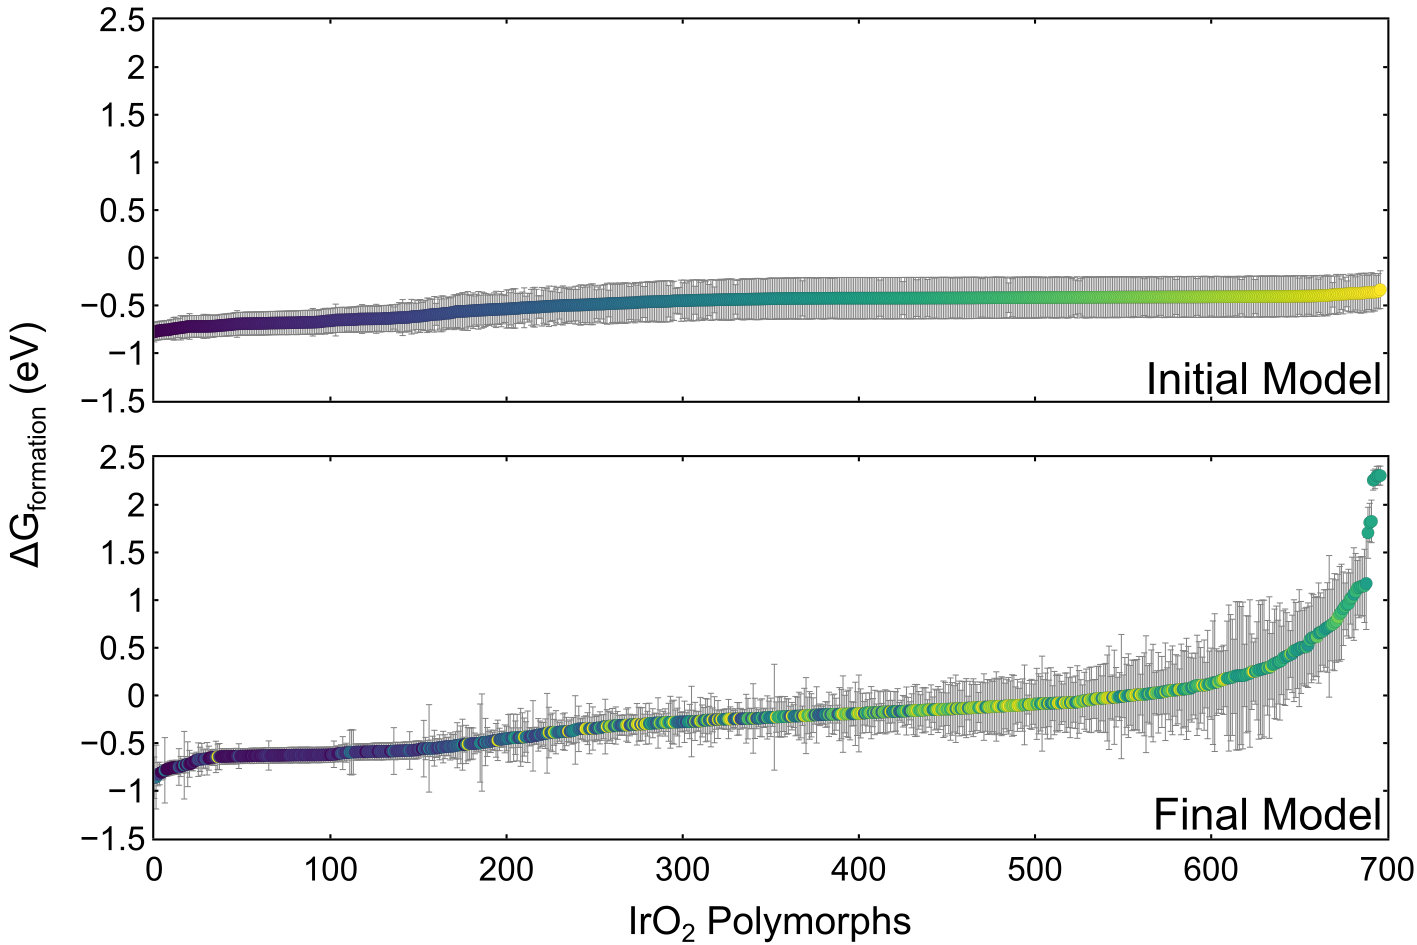
\includegraphics
  {02_figures/ml_convergence_plots/00_master__iro2-ml-conv_v1__200dpi__0__outplot.png}
  % {02_figures/ml_convergence_plots/iro2_ml_conv.png}
  }
\caption{\label{fig:convergence_plot_iro2_0}
  TEMP.
  }
\end{figure}
% __|


  % - 02.01 | IrO3 ************************************************************
  \subsection{II. \ce{IrO_3}}
  %%%%%%%%%%%%%%%%%%%%%%%%%%%%%%%%%%%%%%%%%%%%%%%%%%%%%%%%%%%%%%%%%%%%%%%%%%%%%%%
%%
%%
%%
%%%%%%%%%%%%%%%%%%%%%%%%%%%%%%%%%%%%%%%%%%%%%%%%%%%%%%%%%%%%%%%%%%%%%%%%%%%%%%%


% ################################# Paragraph #################################
% AB3 Structures and Training
- XYZ unique AB3 Structures, 259 unique prototypes.  Substitute Ir and O, expand to minimum Ir-O distance > XYZ
- followed same procedure as in 3.1, Training Set of 35 structures, 8 of which are \ce{IrO_3}
- Describe initial training and training after first 10 DFT structures

% ################################# Paragraph #################################
% P2 Analysis of \ce{IrO_3} Structures
% #COMBAK Change alpha to actual greek symbol
- Describe convex hull, classes of structures (\ce{$\alpha$-AlF3} like, rutile like, and layered, should be segregated in hull plot)
- briefly describe structures within each class, cite in literature where appropriate

  % | - Figure | IrO3 Convergence Plot
\begin{figure}
\centering
\makebox[\textwidth][c]{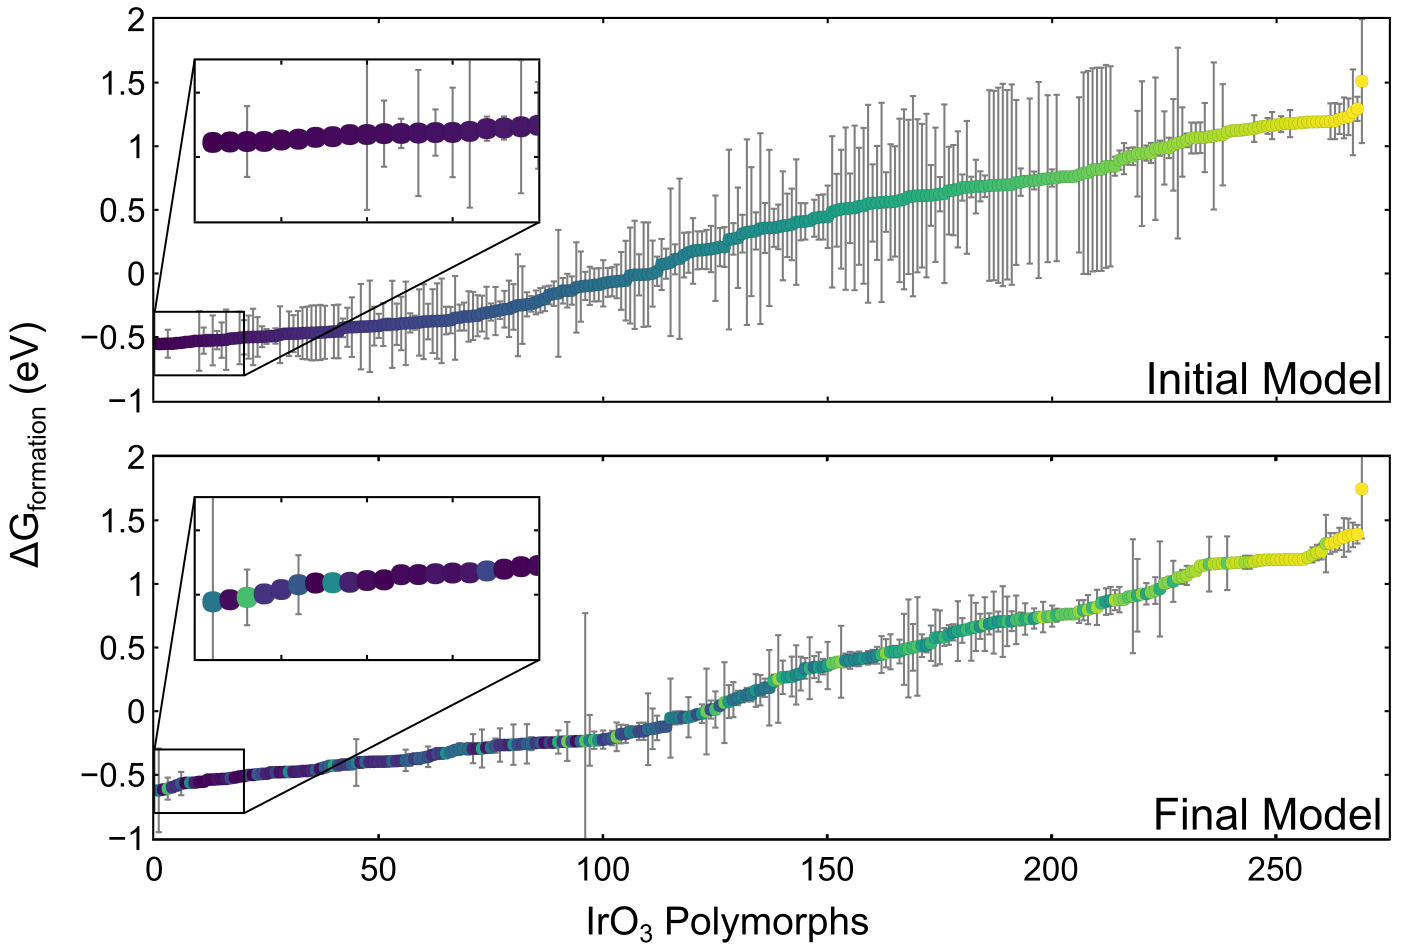
\includegraphics
  {02_figures/ml_convergence_plots/00_master__iro3-ml-conv_v6__200dpi__0__outplot.png}
  % {02_figures/ml_convergence_plots/iro3_ml_conv.png}
  }

\caption{\label{fig:convergence_plot_iro3_0}
  TEMP.
  }
\end{figure}
  % __|


  % - 02.02 | Electrochemical OER Application *********************************
  \subsection{III. Electrochemical OER Application}
  %%%%%%%%%%%%%%%%%%%%%%%%%%%%%%%%%%%%%%%%%%%%%%%%%%%%%%%%%%%%%%%%%%%%%%%%%%%%%%%
%% Electrochemical OER Application
%%
%% TODO: Put (s) on a-IrO3 phase in bulk Pourbaix diagram
%%%%%%%%%%%%%%%%%%%%%%%%%%%%%%%%%%%%%%%%%%%%%%%%%%%%%%%%%%%%%%%%%%%%%%%%%%%%%%%


% ################################# Paragraph #################################
% %%%%%%%%%%%%%%%%%%%%%%%%%%%%%%%%%%%%%%%%%%%%%%%%%%%%%%%%%%%%%%%%%%%%%%%%%%%%%
% TEMP
% %%%%%%%%%%%%%%%%%%%%%%%%%%%%%%%%%%%%%%%%%%%%%%%%%%%%%%%%%%%%%%%%%%%%%%%%%%%%%
% Short introduction into the cataylsis section
In the following section we will demonstrate the merit of our stable polymorph discovery algorithm by elucidating the electrochemical properties of the four promising structures discussed in the previous section.
In particular, surfaces constructed from the four polymorphs will be evaluated for their activity towards the oxygen evolution reaction (OER), an important chemistry with direct application to fuel cell devices.
Additionally, the surfaces will be evaluated for their stability and equilibrium surface coverage of surface oxygen and hydroxides.

% | - Bulk Pourbaix
\subsubsection{Bulk Pourbaix}

% ################################# Paragraph #################################
% %%%%%%%%%%%%%%%%%%%%%%%%%%%%%%%%%%%%%%%%%%%%%%%%%%%%%%%%%%%%%%%%%%%%%%%%%%%%%
% #COMBAK
% #QUESTION Use E or U for potential variable
% %%%%%%%%%%%%%%%%%%%%%%%%%%%%%%%%%%%%%%%%%%%%%%%%%%%%%%%%%%%%%%%%%%%%%%%%%%%%%
The electrochemical stability phase diagram (E vs. pH) was constructed by considering the equilibrium conditions of the following species: Ir, \rIrOtwo, \aIrOthree,  \rIrOthree, \bIrOthree, and an aqueous dissolved \ce{IrO[4-]} species (See TEMP|SI for additional details).
The resulting diagram is shown in Fig. \ref{fig:bulk_pourbaix}.
Importantly, under acidic conditions (pH \textless 7) and in the bias region of interest for the OER (~1.23 V vs. RHE) \aIrOthree shows a large window of stability.
This indicates that the \aIrOthree phase may be stabilized under the highly oxidizing conditions of the OER.
For comparison, the stability regions of the metastable \rIrOthree and \bIrOthree phases, in the absence of any other competing \ce{IrO_3} polymorphs, are indicated by unfilled solid lines.
As shown, these metastable phases appear to also have a wide region of stability in the OER region,
due to to their formation energies being within TEMP eV of the globally stable \aIrOthree phase, see SI table TEMP for the bulk energies of all considered phases.
Because of their similar energies it is possible that some or all of these \ce{IrO_3} phases may be present and relevent for the OER.
In the next section, we explore this possibility by computing the theoretical OER activity of these polymorph systems.
% Also explain the Ir and IrO[4-] ion

% | - Figure | Bulk Pourbaix Diagram
\begin{figure*}
\centering
\makebox[\textwidth][c]{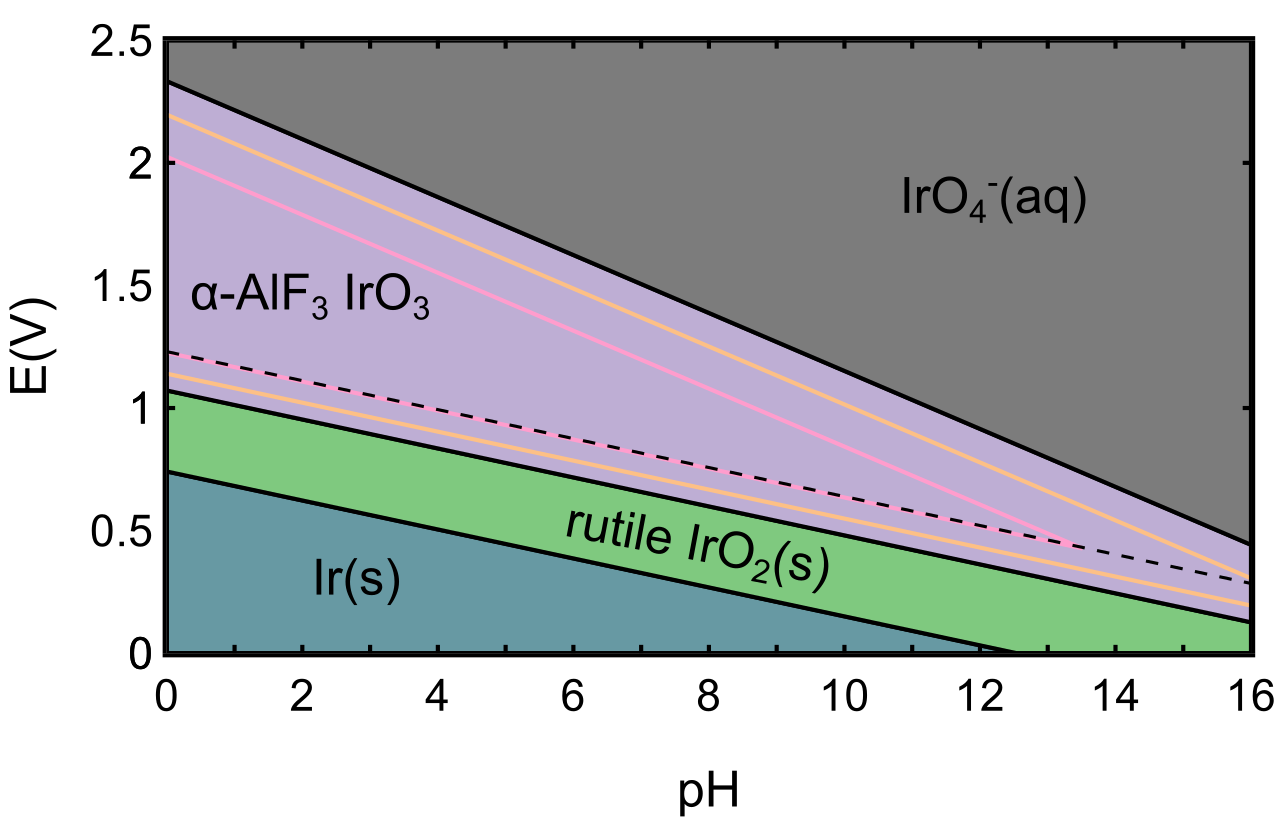
\includegraphics
{02_figures/oer_activity_stability/00_master__bulk-pourbaix__v1__400dpi__0__outplot.png}
% {02_figures/oer_activity_stability/bulk_pourbaix_0.pdf}
}
\caption{\label{fig:bulk_pourbaix},
Electrochemical bulk phasetability diagram (Pourbaix) of the Ir-O-H chemical space with respects to changes in potential and pH.
We considered a bulk unoxidized Ir(s) (blue), a [+4] \rIrOtwo  (green), and an aqueously dissolved \ce{IrO4[4-]} (grey) phase.
Additionnally, we considered the three \ce{IrO_3} polymorphs, \aIrOthree (purple), \rIrOthree (orange), and \bIrOthree (pink).
The water equilibrium line at 1.23 V vs RHE, which corresponds to a 0 overpotential catalyst, is shown by a dotted line.
}
\end{figure*}
% __|

% __|

% | - OER Activities and Surfaces
\subsubsection{b. OER Activities and Surfaces}

% ################################# Paragraph #################################
% %%%%%%%%%%%%%%%%%%%%%%%%%%%%%%%%%%%%%%%%%%%%%%%%%%%%%%%%%%%%%%%%%%%%%%%%%%%%%
% Introduction to OER results
% %%%%%%%%%%%%%%%%%%%%%%%%%%%%%%%%%%%%%%%%%%%%%%%%%%%%%%%%%%%%%%%%%%%%%%%%%%%%%
Fig. \ref{fig:oer_volcano} summarizes the major results of the electrochemical activity and surface stability analysis.
First, Fig. \ref{fig:oer_volcano} a.) shows the surace energy Pourbaix plots for the four IrOx crystals of interest. For each bulk system, the surface energy as a function of applied potential (pH=0), for various facets, and at various coverages (bare, *OH, and *O covered), are shown, see SI for more details.
% How facets were chosen | TODO Get x-ray pattern for systems
% TODO #REF | Reference for VESTA x-ray diff. pattern method
The specific facets were chosen from the highest intensity x-ray diffraction peaks from powder-diffraction spectra simulated in VESTA,
as well as using physical intuition as to which facets would be most physical.
% Say that the IrO3 bulk phase corresponds to the o-covered regime
Additionally, the bulk phase limits of stability from figure TEMP are included at the bottom of each subplot.
In most cases, the oxygen covered surfaces dominate at the OER equilibrium potential (1.23 V vs RHE) with bare surfaces being competitive to within TEMP eV/A2,
this competitivness goes away at even modest overpotentials (eta~0.3, --> ~1.5 V vs RHE),
at which point the oxygen covered terminations are further overstabalized relative to the bare surfaces,
making them the sole dominant termination.
% COMBAK, Revise "mainly" if we include some different coverags
Therefore in our activity analysis we consider mainly oxygen terminated surfaces for the OER.
The OER activity (expressed in terms of the limiting potential) for select oxygen terminated surfaces are shown in Fig. \ref{fig:oer_volcano} as a function of the DGO-DGOH TEMP OER thermodynamic descriptr.
The two rutile-IrO2 suraces (100, and 110) are located towards the strong binding side of the volcano, indicating that that they bind OER intemediate too strongly.
% Reference all experimental IrO2 overpotentials I can find
Encourangly, with predicted overpotentials of TEMP and TEMP, our rutile-IrO2 are within the range of experimental overpotentials found in literature.
The three IrO3 polymorph surfaces all have DGO-DGOH descriptor towards the top and right of the volcano, indicative of weaker binding energetics.
This is evident from figure SI TEMP (scaling) which shows a clear distinction between the IrO2 and IrO3 polymorphs, with IrO3 binding on average TEMP eV weaker than IrO2.
The best performing systems, including the (100), (110), and (211) facets of a-IrO3, b-IrO3 (101), and R-IrO3 (110), have overpotentials of ~0.4 V vs RHE,
a ~0.2 V vs RHE improvemnt over the rutile-IrO2 system.
We note that the computed  overpotentials for our \rIrOtwo system differs from that reported in REFERENCE_Colin_Science by ~0.2 V. This discrepency is due to our us of spin-polarization, which was neglected in Seitz et al., which strenghens the binding of IrO2.


% | - Figure | OER Volcano/Surface Pourbaix
\begin{figure*}
\centering
\makebox[\textwidth][c]{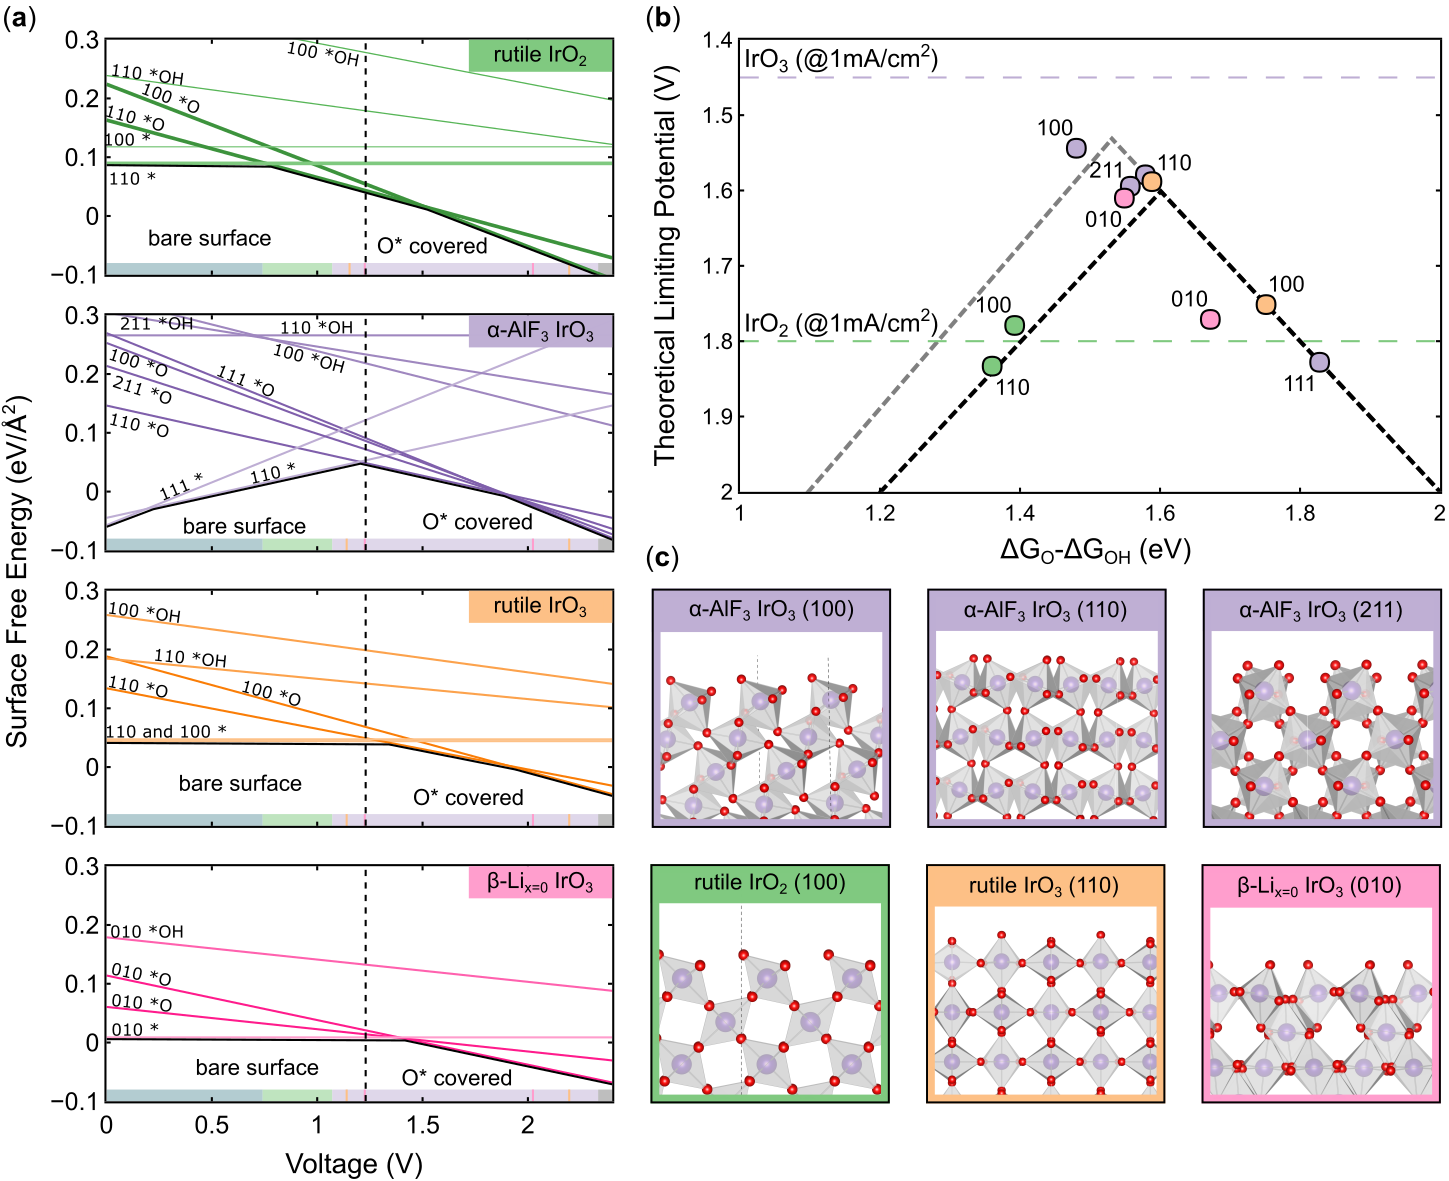
\includegraphics
{02_figures/oer_activity_stability/00_master__oer-volc_surf-pourb_struct__main_v3__200dpi__outplot.png}
% {02_figures/oer_activity_stability/00_master_plot__oer-volc_surf-pourb_struct__main_v3__outplot.pdf}
}
\caption{\label{fig:oer_volcano}
Summary of OER results for the four bulk structures of \IrOx considered: rutile-\ce{IrO_2} (green), $\alpha$-\ce{IrO_3} (purple), rutile-\ce{IrO_3} (orange), and $\beta$-\ce{IrO_3} (pink).
% -----------------------------------------------------------------------------
(a) Surface energy Pourbaix diagrams for each structure, with the surface energy of various facets and coverages shown as a function of applied potential.
The bulk Pourbaix diagram's bounds of stability at pH 0 are superimposed at the bottom of each subplot.
% -----------------------------------------------------------------------------
(b) OER activity volcano for \IrOx systems considered utilizing the \DGOmOH thermodynamic descriptor.
The purple dotted line corresponds to the experimental limiting potential at 10 mA cm\textsuperscript{2} for \ce{IrO_3}, % #TODO #REF Insert Seitz Science reference
while the green band corresponds to the range of experimentally observed overpotentials for pristine \ce{IrO_2} catalysts.  % TODO Insert green band into figure
% -----------------------------------------------------------------------------
(c) Select surface facets for the four \IrOx crystal systems considered.
% -----------------------------------------------------------------------------
% | - __old__
% Circles designate oxygen covered surfaces while triangles designate hydroxyl (*OH) terminated surfaces (relevant surface terminations were found via surface Pourbaix analyses).
% Surface energies at standard conditions (pH and V = 0) are reflected in the border color for each data point, where black indicates a low energy surface termination and white indicates more unstable surfaces.  % Currently not implemented as this
% The color range goes from x to y.
% __|
}
\end{figure*}
% __|

% __|

% | - OER Scaling Relations | TODO | MOVE THIS TO SI
\subsubsection{c. OER Intermediate Scaling}

% ################################# Paragraph #################################
% %%%%%%%%%%%%%%%%%%%%%%%%%%%%%%%%%%%%%%%%%%%%%%%%%%%%%%%%%%%%%%%%%%%%%%%%%%%%%
% TEMP
% %%%%%%%%%%%%%%%%%%%%%%%%%%%%%%%%%%%%%%%%%%%%%%%%%%%%%%%%%%%%%%%%%%%%%%%%%%%%%
Figure TEMP shows the scaling relations between the adsorption free energies of the OER intermediate species for the \IrOx systems studied herein.
It can be seen clearly that the data points corresponding to the three \ce{IrO_3} polymorphs are roughly 1 eV weaker binding than the rutile-\ce{IrO_2} points.
This generally weaker binding of the \ce{IrO_3} stoichiometry is responsible for the observed improvement in theoretical activity.
The \DGOOH vs.\DGOH relationship is very close to the traditional ``universal scaling relations'', demonstrating that our materials do not break the infamous \DGOOH vs. \DGOH scaling.

% | - Figure | OER Scaling Relations
\begin{figure*}
\centering
\makebox[\textwidth][c]{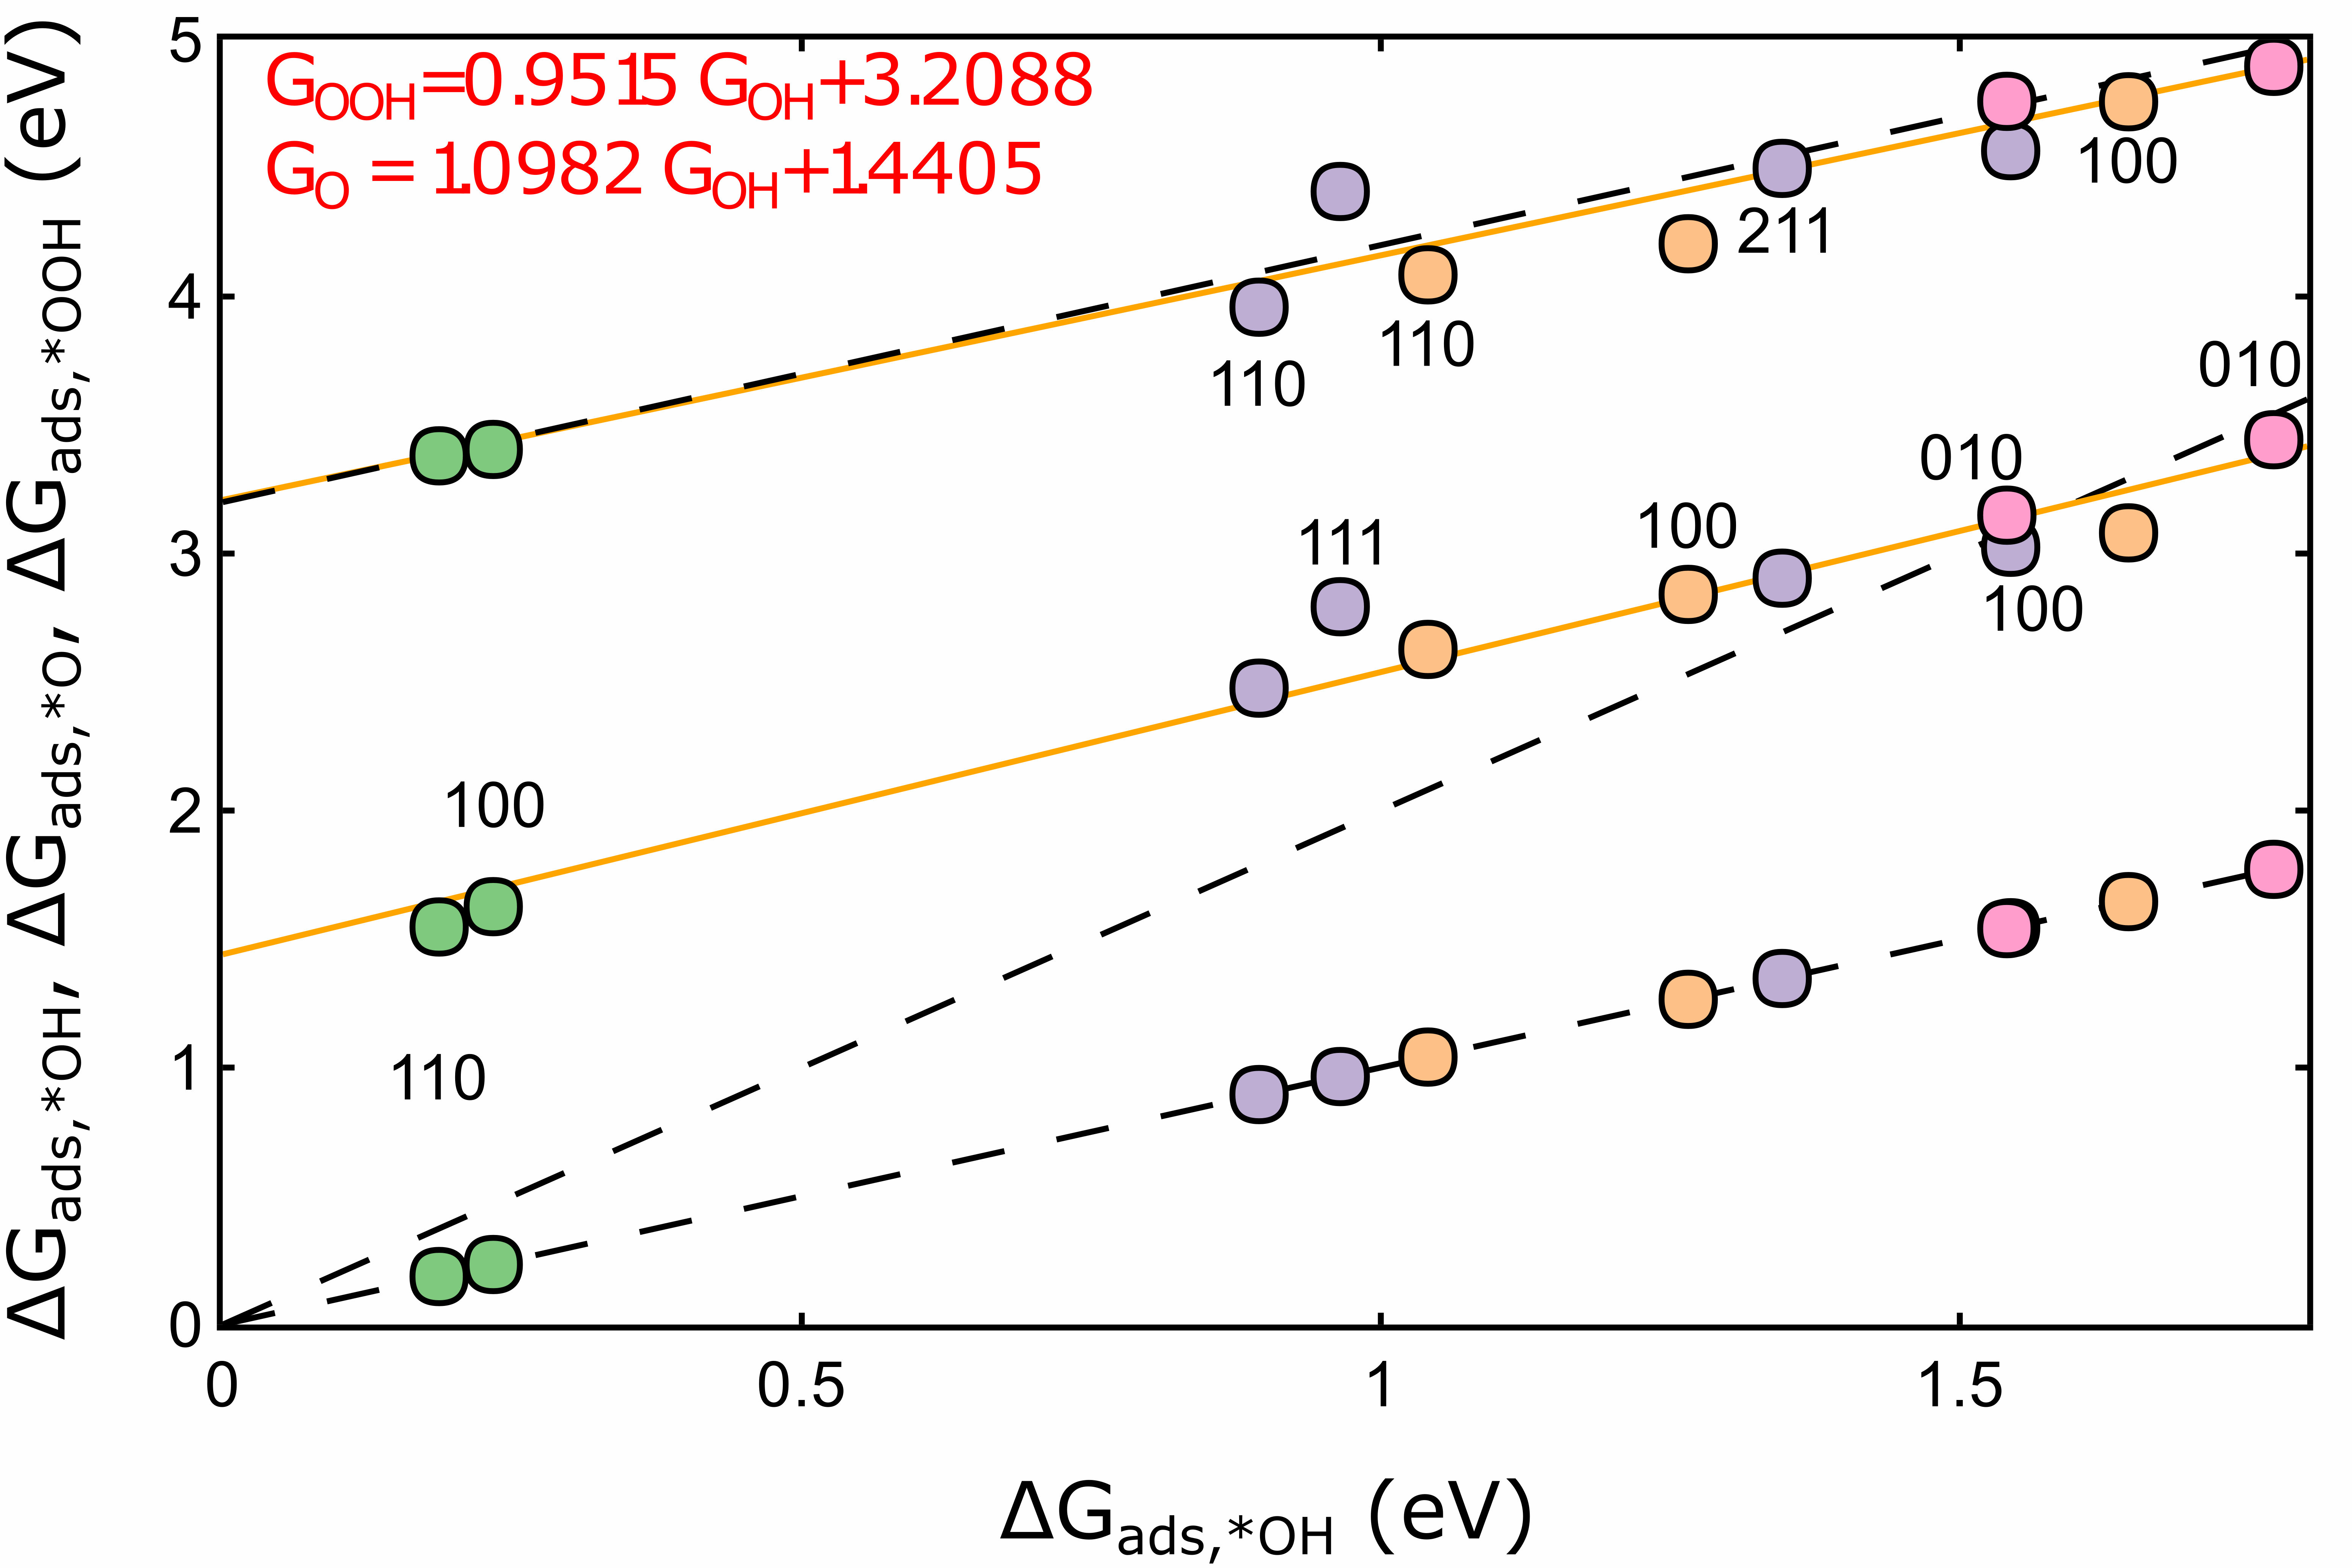
\includegraphics
{02_figures/oer_activity_stability/00_master__oer_scaling__main_v0__outplot2.png}
% {02_figures/oer_activity_stability/pl_scaling_relations_tmp.pdf}
}
\caption{\label{fig:scaling_relations}
% Adsorption free energy scaling relations plot.
Relationship between the adsorption free energies of the three key OER intermediates (*OH, *O, *OOH), with \DGOH chosen as the dependent variable.
Best fit lines are provided for \DGOOH vs. \DGOH and \DGO vs. \DGOH.
Additionally, ``universal scaling relations'' for \DGOOH vs. \DGOH and \DGO vs. \DGOH are shown (black dotted lines) to emphasize our deviation from the traditionally reported scaling fits.
The trivial \DGOH vs. \DGOH relationship is included for completeness.
% TODO Do I have to redefine the color convention every caption?
}
\end{figure*}
% __|

% __|


% - 03 | Conclusion ***********************************************************
\section{Conclusion}
% %%%%%%%%%%%%%%%%%%%%%%%%%%%%%%%%%%%%%%%%%%%%%%%%%%%%%%%%%
% | - Conclusions
% TEMP
% __|
% %%%%%%%%%%%%%%%%%%%%%%%%%%%%%%%%%%%%%%%%%%%%%%%%%%%%%%%%%


% \textbf{Points our results address that are raised in the intro:}

% %%%%%%%%%%%%%%%%%%%%%%%%%%%%%%%%%%%%%%%%%%%%%%%%%%%%%%%%%
% | - PARAGRAPH HEADER
% Conclusions on AL and results
% __|
% %%%%%%%%%%%%%%%%%%%%%%%%%%%%%%%%%%%%%%%%%%%%%%%%%%%%%%%%%
% | - PARAGRAPH BODY
%
% \textbf{Generation of structurally diverse search space and efficient sampling of it.}
We have described a cogent procedure for generating and searching a structurally diverse candidate space of bulk structural prototypes with a desired composition.
%
Once this space is enumerated, we show how it can can be efficiently searched using an algorithm with an active learning loop without a prior knowledge of accurate atomic positions.
%
In most cases, the DFT optimization of only a fraction of the candidates leads to identification of the most stable polymorphs.
%
In particular, this approach is well-suited for discovery in structurally diverse structures, such as metal oxides and other metal-ligand bulk systems, where there exits a large degree of structural diversity.
%
The current dataset includes octahedral, tetrahedral, square-pyramidal, cubic, and square-planar Ir-O conformers.
%
We also note, that our AL algorithm is capable of discovering experimentally known phases such as pyrite, columbite and layered \IrOtwo and several recently discovered layered \IrOthree phases formed by Li$^+$ deintercalation.
%
In particular, we have identified a number of previously unknown \IrOthree polymorphs below the amorphous synthesizability limit,
including a new globally stable \aIrOthree phase.
%
This high valency Ir$^{6+}$ phase is stable under OER relevant conditions and has an ideal 100\% corner-sharing octahedral structure, a short Ir-O bond length of 1.93 \angstrom, and also has a very high surface coverage of active oxygens.
%
Calculations of surface thermodynamics reveal this structure and other OER stable \IrOthree phases have much higher theoretical OER activity than a benchmark rutile \IrOtwo.
%
The thermodynamic stability and high OER activity of the \aIrOthree phase may provide clues as to the nature of the yet uncharacterized structures reported after reconstruction of \ce{SrIrO_{3}} and \IrOx precursors under OER reaction conditions.
%
Methods combining diverse structural generation, AL-enabled accelerated searches, and \mbox{ab-initio} simulation of material performance could open up new avenues for in silico material design with application tailored structural properties.
% __|
% %%%%%%%%%%%%%%%%%%%%%%%%%%%%%%%%%%%%%%%%%%%%%%%%%%%%%%%%%







% | - __old__

% In conclusion, we have demonstrated an active learning accelerated algorithm for the discovery of stable crystal polymorphs by searching through a candidate space of structurally distinct iridium-oxide phases.
% %
% % TODO Can I generalize this result for both IrO2 and IrO3?
% % TODO Use percentage of total systems instead of just # of DFT calcs
% The algorithm can identify a majority of the most stable polymorphs (7 of the 10 most stable) in a candidate set after only computing a fraction of them via DFT (\mytilde90 DFT optimizations).
% %
% For \IrOtwo, we find confirm the rutile phase as the most stable crystal structure, while also finding several well known phases, including anatase, columbite, as well as several new phases of \IrOtwo.
% %
% For the relatively unexplored \IrOthree we found a new globally stable phase (\aIrOthree), a completely corner sharing octahedral structure with space group 182.
% %
% % Implications for for future studies of polymorphs
% %
% % Describe the level of acceleration achieved, effect of structural drift, implications for future studies
% We have analyzed the local and global structural coordination and revealed that octahedral coordination environments are predominantly preferred, although we also have a large degree of structural diversity in our dataset (octahedral, tetrahedral, square-pyramidal, cubic, and square-planar are all represented)
% %
% % Discuss the differences connectivity/M-O bonds lengths is different between IrO2 and IrO3
% %
% We constructed a revised bulk Pourbaix diagram for Ir-H$_2$O, including the newly found \aIrOthree phase and revealed that \aIrOthree has a substantial window of stability in the OER relevant potentials and pH.


% __|


% #############################################################################

% - Acknowledgment ***********************************************************
\begin{acknowledgement}

% COMBAK | Add to, and finalize this
Organizations to acknowledge
TRI
SUNCAT
Stanford
NERSC
etc.

% NOTE | Copied and pasted from some sample text @Michal sent me
JAGT and MB acknowledge the support by the U.S. Department of Energy, Office
of Science, Office of Basic Energy Science, via Grant DE-SC0008685 to the
SUNCAT Center of Interface Science and Catalysis.

The authors would like to acknowledge the use of the computer time allocation
for the “Transition metal-oxide and metal surfaces: applications and
reactivity trends in catalysis” at the National Energy Research Scientific
Computing Center, a DOE Office of Science User Facility supported by the
Office of Science of the U.S. Department of Energy under Contract No.
DE-AC02-05CH11231.

\end{acknowledgement}

% - Supplementary Information *************************************************
% | - __latex_setup__
\clearpage
\appendixhttps://www.overleaf.com/project/5d30a91110dda51a44b9fec4
\renewcommand{\thefigure}{S\arabic{figure}}
\setcounter{figure}{0}
\renewcommand{\thetable}{S\arabic{table}}
\setcounter{table}{0}
% __|

\begin{suppinfo}
%%%%%%%%%%%%%%%%%%%%%%%%%%%%%%%%%%%%%%%%%%%%%%%%%%%%%%%%%%%%%%%%%%%%%%%%%%%%%%%
%%
%%
%%
%%%%%%%%%%%%%%%%%%%%%%%%%%%%%%%%%%%%%%%%%%%%%%%%%%%%%%%%%%%%%%%%%%%%%%%%%%%%%%%


% | - Machine Learning Algorithm Methods
\subsection{Machine Learning Algorithm Methods}

Relevant details about the ML Gaussian process here % @Chris
% __|

% | - Electrochemical OER Computational Methods
\subsection{Electrochemical OER Computational Methods}

% | - Density Functional Theory Methods
\subsubsection{Density Functional Theory Methods}
% Get VASP #REF in the ex. word doc. that @Michal shared with me
All OER calculations were performed using density functional theory (DFT) implemented via the Vienna ab-initio simulation package (VASP) and utilizing the PBE exchange-correlation functional.
Dipole corrections were imposed on all non-symmetric slabs.
A 4x4x3 k-point mesh with gamma-point centered Monkshort-packing was used for all slabs.
The plane-wave energy cutoff was 500 eV.

% COMBAK Figure out how much spacing was used for all slabs
% FIXME Change the A -> Angstrom symbol

% COMBAK What kind of optimization routine was used? (Newtonian, BFGS?)
All slab calculations maintained a vacuum spacing of <15 A.
% COMBAK change A -> Angstrom
All structures were relaxed utilizing a TEMP algorithm with a stop criteria being that all atoms satisfy a maximum force threshold of 0.02 eV/A.
% __|

% | - OER Thermodynamic Methodology
\subsubsection{OER Thermodynamic Methodology}
% __|

% | - Surface Energy Pourbaix Methodology
\subsubsection{Surface Energy Pourbaix Methodology}
% __|

Procedure:
- For the top/most stable bulk structures the following procedure was carried out

* Stable stoicheometric terminations were cut from the bulk
    Stable termination planes were guesstimated via intuition, and the x-ray diffraction pattern tool from Vesta

* Electrochemical surface coverage was elucidated via a surface Pourbaix analysis
    Need to know the coverage of surface under operating conditions (>1.23 V RHE)

* Thermodynamic/limiting potential analysis of the OER mechanistic pathway
    Volcano plot, limiting potentials, etc.

% TODO Gibbs corrections, OER mechanism
% __|

\end{suppinfo}

% Bibliography ****************************************************************
\bibliography{01_references/dummy_refs.bib}

\end{document}
